%input macros (i.e. write your own macros file called MacroFile1.tex)
%\newcommand{\PdfPsText}[2]{
  \ifpdf
     #1
  \else
     #2
  \fi
}

\newcommand{\IncludeGraphicsH}[3]{
  \PdfPsText{\includegraphics[height=#2]{#1}}{\includegraphics[bb = #3, height=#2]{#1}}
}

\newcommand{\IncludeGraphicsW}[3]{
  \PdfPsText{\includegraphics[width=#2]{#1}}{\includegraphics[bb = #3, width=#2]{#1}}
}

\newcommand{\InsertFig}[3]{
  \begin{figure}[!htbp]
    \begin{center}
      \leavevmode
      #1
      \caption{#2}
      \label{#3}
    \end{center}
  \end{figure}
}


%%% Local Variables: 
%%% mode: latex
%%% TeX-master: "~/Documents/LaTeX/CUEDThesisPSnPDF/thesis"
%%% End: 


 \documentclass[oneside,12pt]{CUEDthesisPSnPDF}


\ifpdf
    \pdfinfo { /Title  (Congestion Control Mechanisms for Optical Burst Switched Networks)
               /Creator (TeX)
               /Producer (pdfTeX)
               /Author (Fei Wang fei.wang2@mail.dcu.ie)
               /CreationDate (D:20110417000000)  %format D:YYYYMMDDhhmmss
               /ModDate (D:20110417000000)
               /Subject (Congestion Control Mechanisms for Optical Burst Switched Networks)
               /Keywords (Congestion Control,OBS)}
    \pdfcatalog { /PageMode (/UseOutlines)
                  /OpenAction (fitbh)  }
\fi

\title{Congestion Control Mechanisms for \\ Optical Burst Switched \\ Networks}

\ifpdf
  \author{Fei Wang}
  \collegeordept{School of Electronic Engineering}
  \university{Dublin City University}
% insert below the file name that contains the crest in-place of 'UnivShield'
  \crest{
\includegraphics[width=30mm]{UnivShield}}
  \supervisor{Dr. Conor McArdle}
\else
  \author{Fei Wang}
  \collegeordept{School of Electronic Engineering}
  \university{Dublin City University}
% insert below the file name that contains the crest in-place of 'UnivShield'
  \crest{
\includegraphics[bb = 0 0 292 336, width=30mm]{UnivShield}}
\fi
%
% insert below the file name that contains the crest in-place of 'UnivShield'
% \crest{\IncludeGraphicsW{UnivShield}{40mm}{14 14 73 81}}
%
%\renewcommand{\submittedtext}{change the default text here if needed}
\degree{TELECOMMUNICATIONS}
\degreedate{Apirl 2011}

% turn of those nasty overfull and underfull hboxes
\hbadness=10000
\hfuzz=50pt

% Put all the style files you want in the directory StyleFiles and usepackage like this:
\usepackage{watermark}
\usepackage{array}
\usepackage{multirow}
% Comment out the next line to get single spacing
\onehalfspacing

\usepackage[parfill]{parskip}

\begin{document}
%\language{english}

% A page with the abstract on including title and author etc may be
% required to be handed in separately. If this is not so, then comment
% the below 3 lines (between '\begin{abstractseparte}' and 
% 'end{abstractseparate}'), normally like a declaration ... needs some more
% work, mind as environment abstracts creates a new page!
% \begin{abstractseparate}
%   
% Thesis Abstract -----------------------------------------------------


%\begin{abstractslong}    %uncommenting this line, gives a different abstract heading
\begin{abstracts}        %this creates the heading for the abstract page

    In this studies, I review burst congestion control problems in optical burst switching networks from the viewpoint of network throughput maximizaation and to reduce additional signal requirement while minimizing burst loss. Burst collision occurs when two or more bursts access the same wavelength at the same time, and the occurrence becomes more frequent with the offered load increases. 
    Burst must be dropped since OBS don't provide buffer on intermediate core router. That is said contention is inherent to the OBS network. There are a lot of predecessors have done a lot of research on this topic. General speaking, it has two jointly operating mechanisms, namely a burst congestion detection and a burst control algorithm. In this work, I want to overcome the shortcoming of previous research and develop a new mechanism to enhace OBS network stability and make
    congestion controllable. 
    \par
    {\bfseries Keyword:} Optical Switching Networks, Congestion Control

\end{abstracts}
%\end{abstractlongs}


% ----------------------------------------------------------------------


%%% Local Variables: 
%%% mode: latex
%%% TeX-master: "../thesis"
%%% End: 

% \end{abstractseparate}


% Using the watermark package which is in StyleFiles/
% and to remove DRAFT COPY ONLY appearing on the top of all pages comment out below line
%\watermark{DRAFT COPY ONLY}


\maketitle
%{\newpage
%\thispagestyle{empty}
%\mbox{}}

%set the number of sectioning levels that get number and appear in the contents
\setcounter{secnumdepth}{3}
\setcounter{tocdepth}{3}
\frontmatter % book mode only

%\pagenumbering{roman}

\renewcommand{\thepage}{\mbox{A-\arabic{page}}}
%\renewcommand{\thefigure}{A-\arabic{figure}}

\renewcommand{\thefigure}{A-\arabic{chapter}.\arabic{figure}}
\renewcommand{\thetable}{A-\arabic{chapter}.\arabic{table}}

%\phantomsection
%\cleardoublepage
%\addcontentsline{toc}{chapter}{Acknowledgement}
%% Thesis Acknowledgements ------------------------------------------------


%\begin{acknowledgementslong} %uncommenting this line, gives a different acknowledgements heading
\begin{acknowledgements}      %this creates the heading for the acknowlegments

First and foremost I offer my sincerest gratitude to my supervisor, Dr. Conor McArdle, who has supported me throughout my thesis with his patience and knowledge whilst allowing me the room to work in my own way. I attribute the level of my Masters degree to his encouragement and effort and without him this thesis,too,would not have been completed or written. One simply could not wish for a better or friendlier supervisor.

Thanks are also due to Prof. Tommy Curran for supporting this work to date,etc. I am also greatly indebted to the professors and teachers at the school of electronic engineering: Dr. Martin Collier, Dr. Jennifer McManis, Dr. Gabriel-Miro Muntean, who have instructed and helped me a lot in the past years. Especially, I would like to express my appreciation to Dr. Derek Molloy for preparing the original version of this template document.   

Last my thanks would go to my beloved family for their loving considerations and great confidence in me all through these years. I also owe my sincere gratitude to my friends and my fellow classmates who gave me their help and time in listening to me and helping me work out my problems during the difficult course of the thesis.

Last but not least, I would like to thank those who relly made it possible for me to do my master at DCU because of their encouragement and emotional support.

\end{acknowledgements}
%\end{acknowledgmentslong}

% ------------------------------------------------------------------------

%%% Local Variables: 
%%% mode: latex
%%% TeX-master: "../thesis"
%%% End: 


\phantomsection
\cleardoublepage
% Thesis Dedictation ---------------------------------------------------

\begin{dedication} %this creates the heading for the dedication page
I hereby declare that, except where otherwise indicated, this document is entirely my own work and has not been submitted in whole or in part to any other university.


\vspace*{5ex}

{Signed:\, \underline{Fei Wang}}
\hspace*{54mm}
{Date:\, \underline{26-Apr-2011}}


\end{dedication}

% ----------------------------------------------------------------------

%%% Local Variables: 
%%% mode: latex
%%% TeX-master: "../thesis"
%%% End: 


\setcounter{page}{2}
\phantomsection
\cleardoublepage
\addcontentsline{toc}{chapter}{Abstract}

% Thesis Abstract -----------------------------------------------------


%\begin{abstractslong}    %uncommenting this line, gives a different abstract heading
\begin{abstracts}        %this creates the heading for the abstract page

    In this studies, I review burst congestion control problems in optical burst switching networks from the viewpoint of network throughput maximizaation and to reduce additional signal requirement while minimizing burst loss. Burst collision occurs when two or more bursts access the same wavelength at the same time, and the occurrence becomes more frequent with the offered load increases. 
    Burst must be dropped since OBS don't provide buffer on intermediate core router. That is said contention is inherent to the OBS network. There are a lot of predecessors have done a lot of research on this topic. General speaking, it has two jointly operating mechanisms, namely a burst congestion detection and a burst control algorithm. In this work, I want to overcome the shortcoming of previous research and develop a new mechanism to enhace OBS network stability and make
    congestion controllable. 
    \par
    {\bfseries Keyword:} Optical Switching Networks, Congestion Control

\end{abstracts}
%\end{abstractlongs}


% ----------------------------------------------------------------------


%%% Local Variables: 
%%% mode: latex
%%% TeX-master: "../thesis"
%%% End: 


\renewcommand\contentsname{Table of Contents}
\tableofcontents
\thispagestyle{empty}
\listoffigures
\thispagestyle{empty}
\listoftables
\thispagestyle{empty}

\input{glossary.tex}
\printnomenclature  %% Print the nomenclature
\thispagestyle{empty}
\addcontentsline{toc}{chapter}{Glossary}

\mainmatter % book mode only
\setcounter{page}{5}
\renewcommand{\thepage}{\mbox{A-\arabic{page}}}
%\renewcommand{\thefigure}{A-\arabic{figure}}
%\pagenumbering{arabic}
%\setcounter{page}{1}
\section{Introduction}

\IEEEPARstart{O}{BS} has been proposed as strong candidate for the next generation
optical internet. OBS can achieve high statistical multiplexing and
provide flexible and dynamic bandwidth allocation required to support
highly dynamic and burst traffic\cite{ref:obs}.  In OBS networks, all input data
are assembled into a burst according to their destination in edge side, referred to
as data burstsd(DB), Shortly before the burst transmission begin, a
burst header cell(BHC) is sent on the control channel that is
processing on electric domain. The control packet BHC which contains 
information such as the destination address, the length of burst, the
number of hops it pass through and the burst offset time. BHC channel
is separated from the data burst channel. It take offset time to let 
the header cell be processed at each intermediate router before the data 
burst arrives. When all router along the path between source and destination 
complete resource reservation. DB can go through the path within whole
high-speed optical domain. The main different difference between an
optical network and a conventional packet switching network are
without optical buffer on the intermediate router. Once the network is congested,
some or all of bursts have to be dropped since bufferless on OBS. 
Hence, contention is inherent to the OBS technique and contention issue 
could affect tremendously the network performance in
terms of burst blocked rate and throughput. Recently, contention and loss
ratio may be reduced by implementing contention resolution policies,
such as time defection (using fiber delay line \cite{ref:fdl}), space 
deflection (using deflection routing \cite{ref:deflect}), and wavelength 
conversion \cite{ref:conversion}. These mechanisms can reduce burst blocked
rate in short-term burst congestion. But if the burst congestion 
lasts longer, the contention resolution policies can't handle any more. 
Some or all conflict bursts must be dropped. And then there are several soft contention
resolution policy can be applied for determining which bursts to drop.

The contention resolution policies are considered as reactive
approaches in the sense that they are invoked after contention occurs.
But also increase the complex implementation issues. An alternative
approach to avoid network contention and reduce burst loss is by proactively
 attempting to prevent network from overload through traffic management. This
paper focus on how to keep the rate of burst blocked rate of a network 
around a controllable level. An ideal congestion control mechanism should
achieve some objectives: enhance the throughput, reduce the average end-to-end burst delay, reduce data burst blocked rate, fair to all users and react timely. Basically, the congestion problem is due to the lack of information at the nodes and the absence of global coordination between the edge nodes and core nodes. As we know, in OBS, all intelligence resides in the edge nodes, which provides the buffer and the processor at the same time on the network. To solve these problems and consider about the feature of OBS, I develop a detect-feedback-react loop congestion control mechanism. 

The rest of the article is organized as follows.Section 2 stats the background of problem 
and related studies. The proposed congestion control scheme is illustrated in Section 3. 
Section 4 presents and analysis the computer experiment results. Finally, I concludes this paper in Section 5.

% \pagebreak[4]
% \hspace*{1cm}
% \pagebreak[4]
% \hspace*{1cm}
% \pagebreak[4]

\chapter{Literature Review}
\ifpdf
    \graphicspath{{Chapter1/Chapter1Figs/PNG/}{Chapter1/Chapter1Figs/PDF/}{Chapter1/Chapter1Figs/}}
\else
    \graphicspath{{Chapter1/Chapter1Figs/EPS/}{Chapter1/Chapter1Figs/}}
\fi

\section{About optical burst network}

\begin{figure}[!htbp]
    \label{fig:obstransstep}
    \begin{center}
        \leavevmode
        \ifpdf
        \resizebox{120mm}{!}{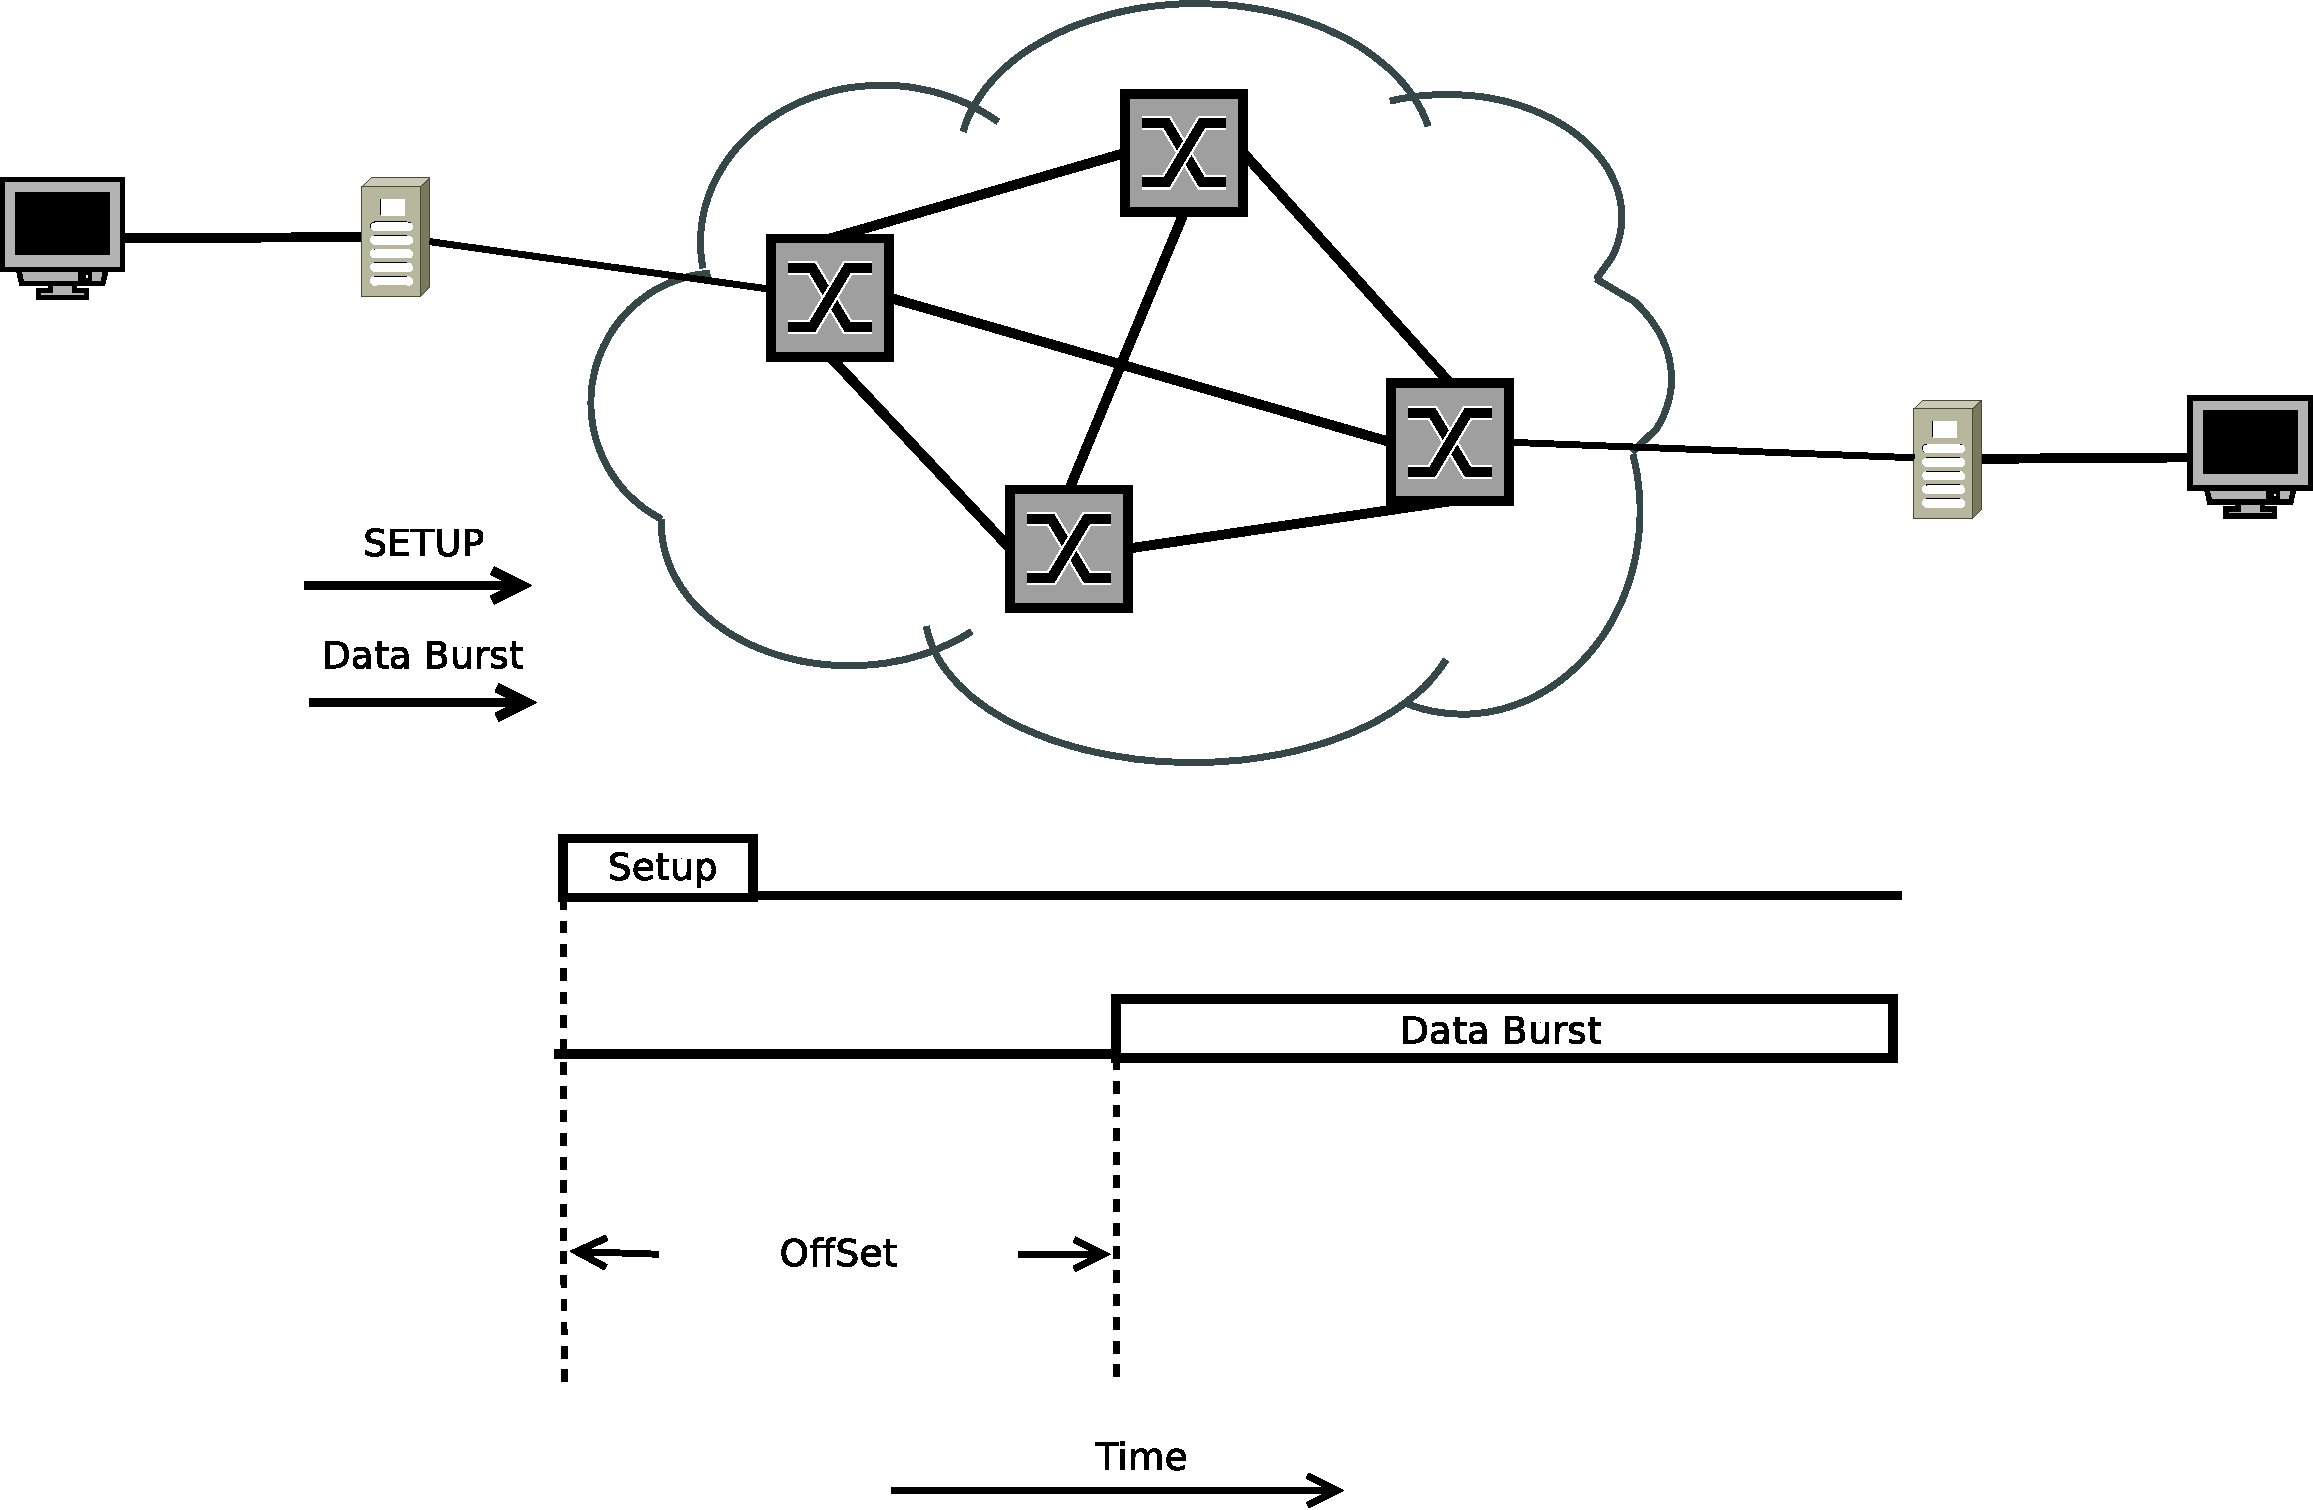
\includegraphics[height=6in]{setup}}
        \else
        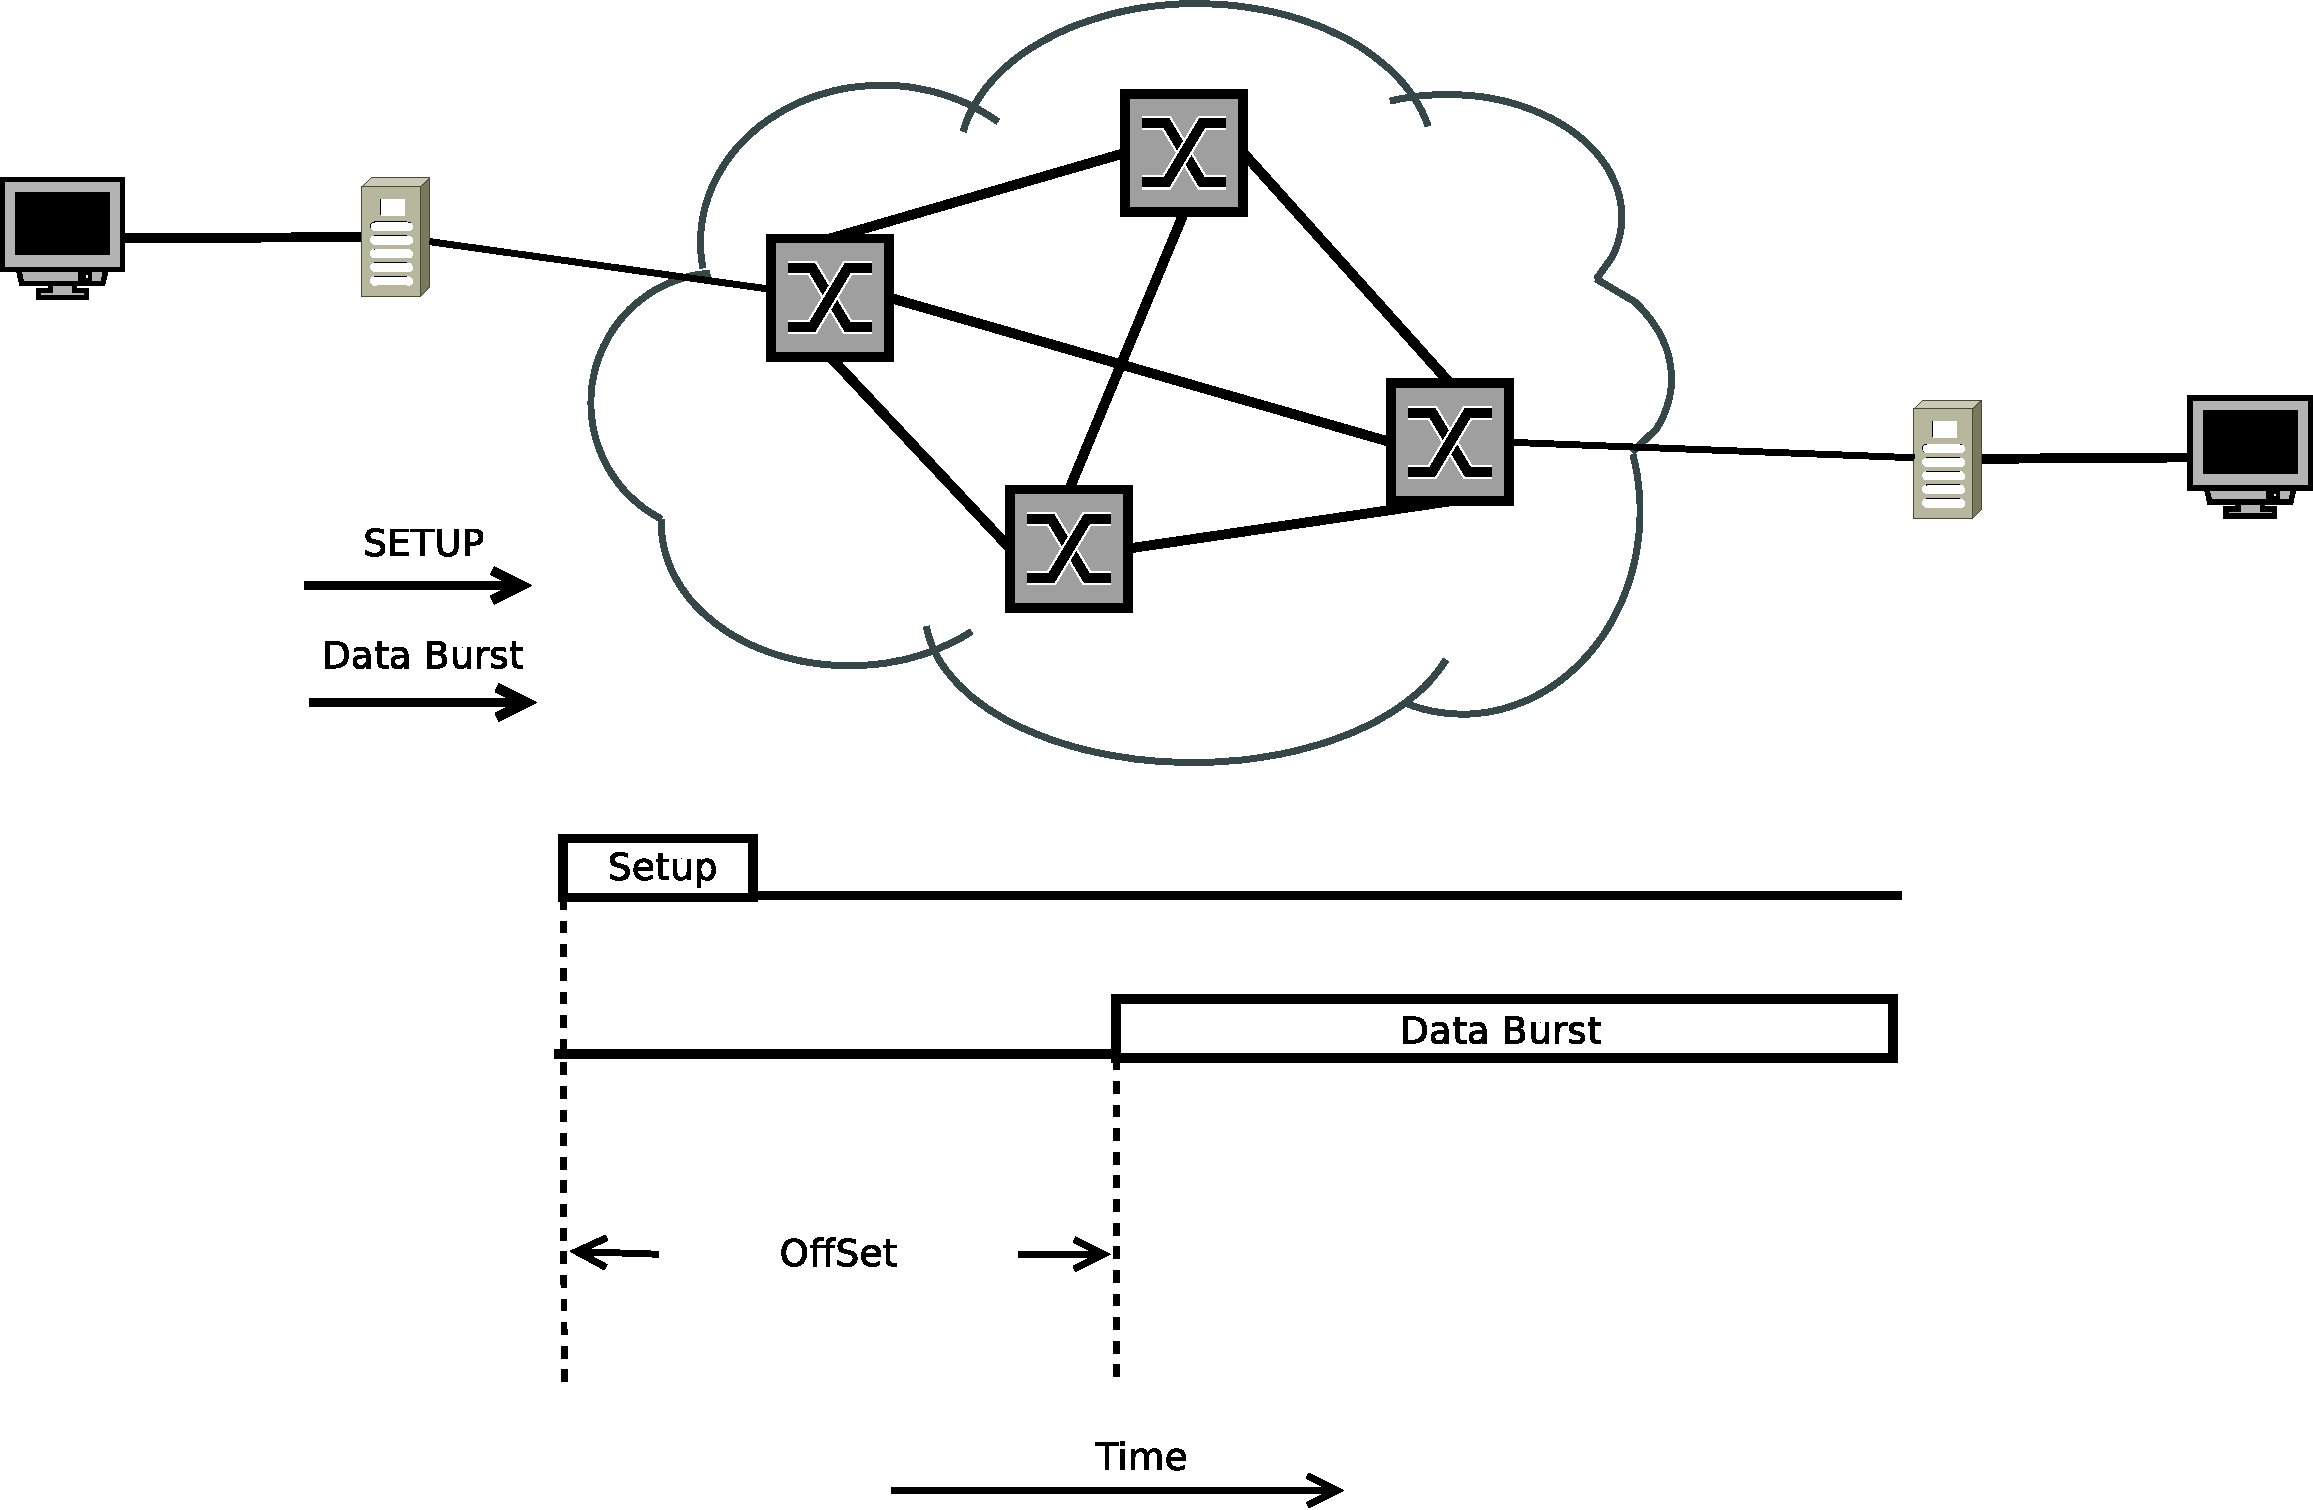
\includegraphics[bb = 92 86 545 742, height=6in]{setup}
        \fi
        \caption{Burst assembly,Burst reservation}
    \end{center}
\end{figure}

Among all optical switching technology, OBS seek to enhance the statistical multiplexing. It has proposed as a new paradigm switching technology for next generation Internet backbone network. Before we get closed to it. We need to get some foundational knowledge, such as what are the big characteristics of this form of exchange of technology. What is the biggest difference compare with traditional switching technology? Does it have born deficiency? 

\begin{figure}[!htb]
    \label{fig:obstime}
    \begin{center}
        \leavevmode
        \ifpdf
        \resizebox{120mm}{!}{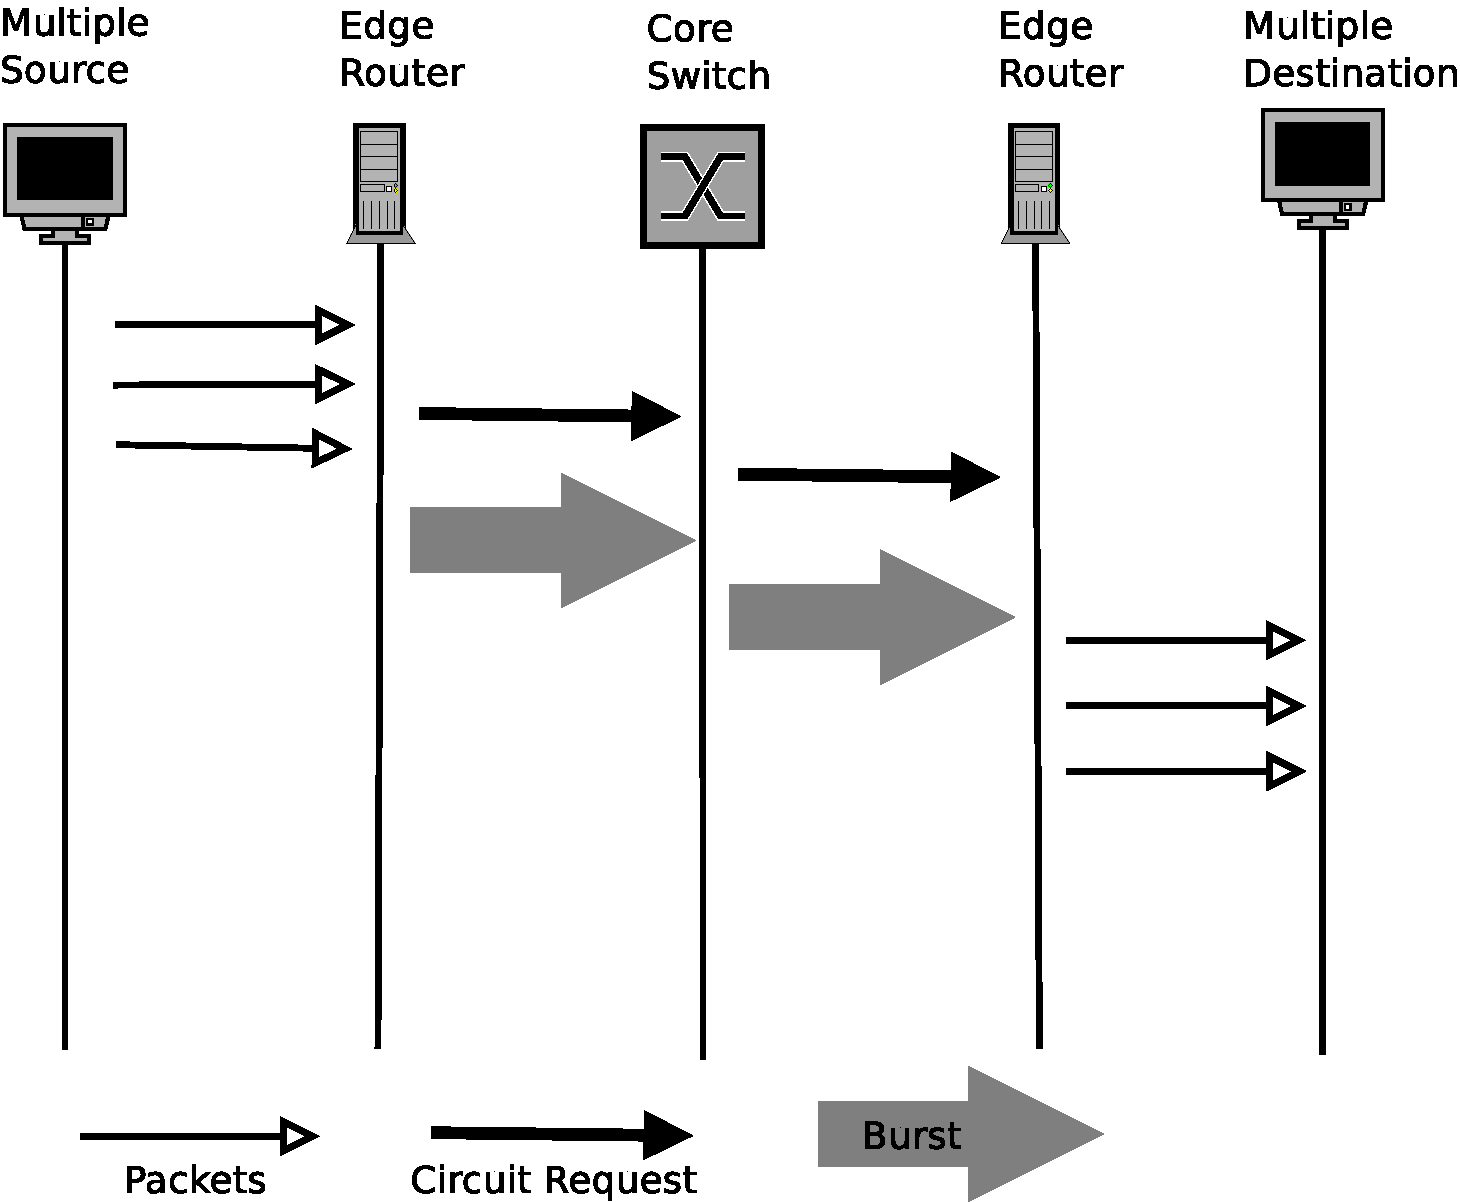
\includegraphics[height=6in]{burst}}
        \else
        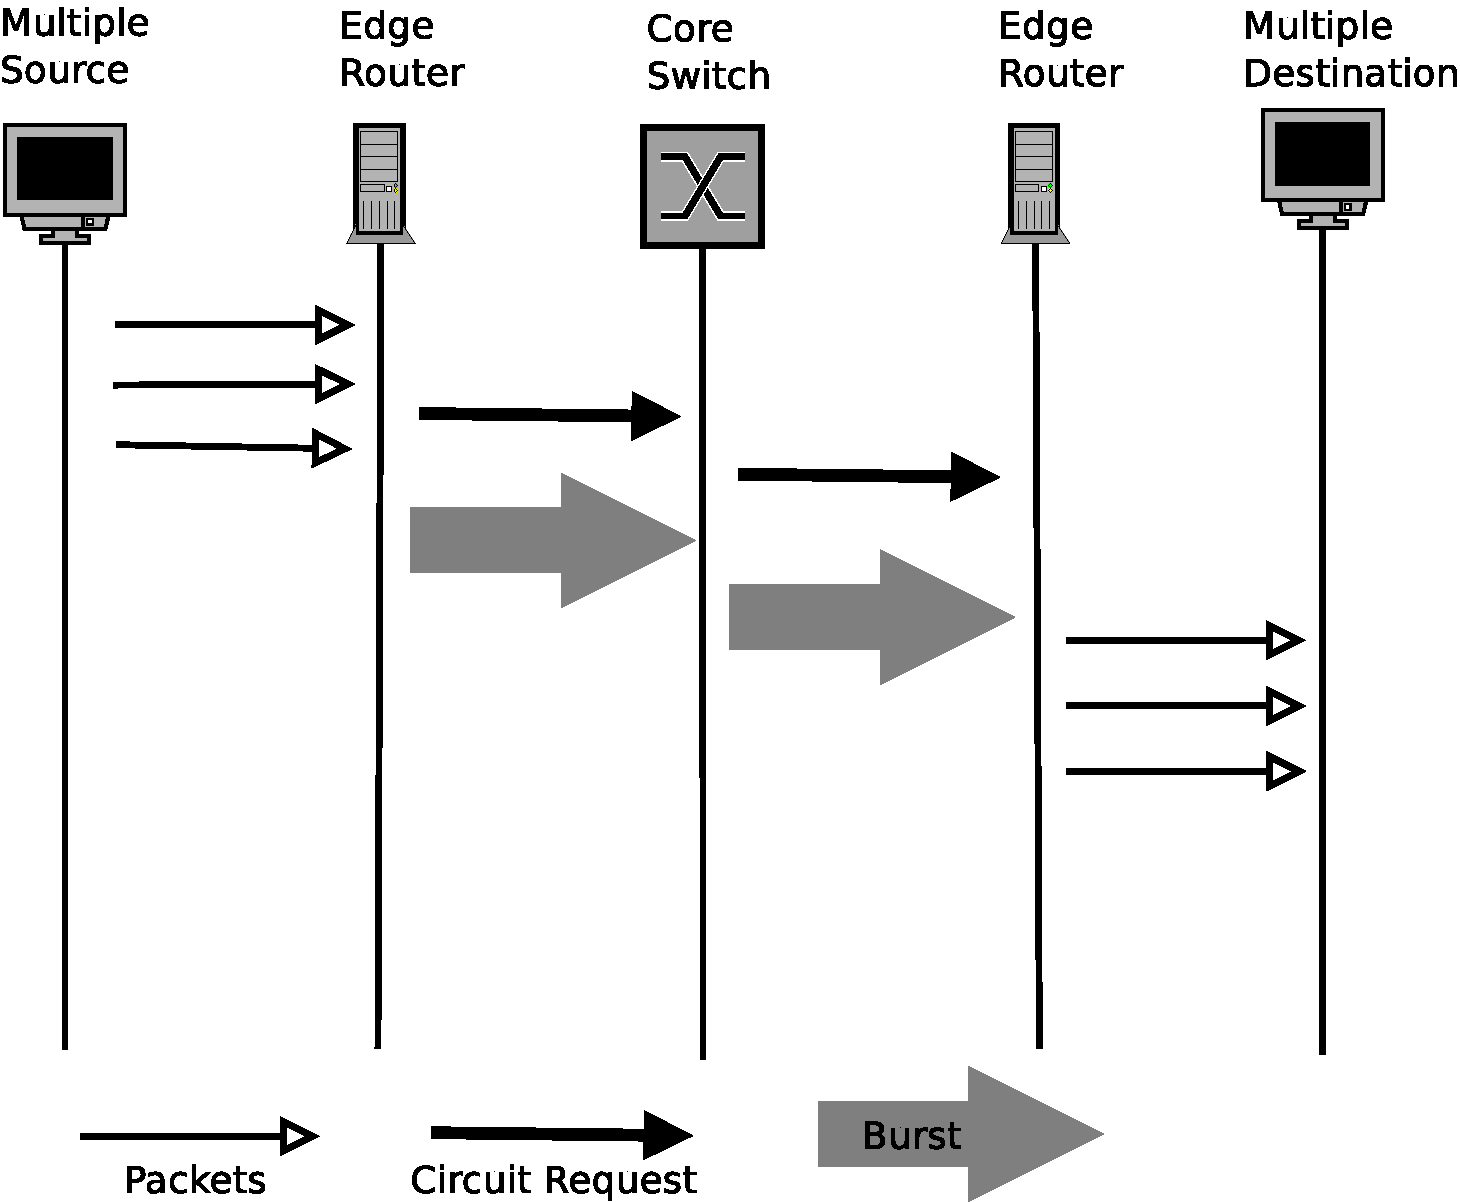
\includegraphics[bb = 92 86 545 742, height=6in]{burst}
        \fi
        \caption{Sample time diagram of a network using OBS}
    \end{center}
\end{figure}

\begin{figure}[!htb]
    \label{fig:burst_format}
    \begin{center}
        \leavevmode
        \ifpdf
        \resizebox{50mm}{!}{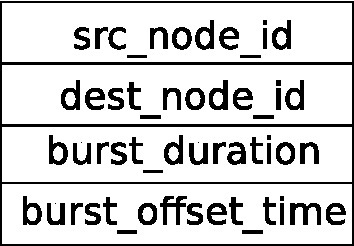
\includegraphics[height=6in]{burst_format}}
        \else
        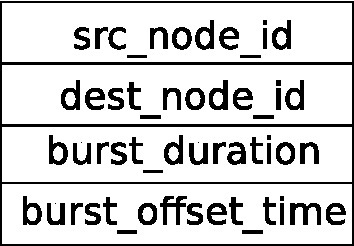
\includegraphics[bb = 92 86 545 742, height=6in]{burst_format}
        \fi
        \caption{OBS burst format sample}
    \end{center}
\end{figure}

The main different compare to conventional packet switching is bufferless on core node. OBS put all intelligent such as buffer, electronic processor, to edge side. As figure \ref{fig:obstransstep} show. All input data bursts are collected into bursts. There may be a classifier to classify packet to different burst according to their destination and Qos requirement or something else. After complete burst assemble and before the burst
transmission begins, a Burst Header Cell (BHC) is sent on the control channel that is separate from data burst channel, carry information about the destination of the burst, duration of the burst, the number of hops it pass through. A sample burst format is shown in figure \ref{fig:burst_format}

A burst switcher, once receiving the BHC, schedule and determine an outgoing link for leading toward the desired destination with an idle channel available, and
then establishes a connection between the channel specified in BHC and the channel through schedule algorithm by core switcher to transmit the burst. It also pass the BHC to next hops on the control channel of the selected link. After the core router prepare for arriving burst, the burst go through core router without additional operation. It also refer as one-way reservation. The burst just wait a certain offset time and don't need to check the ACK from reservation process. Once
burst arrive to core router, It can be transmit in whole optical domain. That is the reason why OBS better than others mechanism. The mechanism for resource reservation and release has been study for a long time. In simple term, There are four major combinations as table \ref{tab:setupclass} show.

\begin{table}[!htbp]
    \label{tab:setupclass}
    \centering
    \setlength{\extrarowheight}{1mm}
    \addtolength{\tabcolsep}{3mm}
    \begin{tabular}{|r|l|l|}
        \hline
        \backslashbox{release}{setup} & Immediate setup & Delay setup \\
        \hline
        \multirow{2}{*}{Immediate release} & Immediate setup & Delay setup\\
                                           & Immediate release & Immediate release\\
        \hline  
        \multirow{2}{*}{Explicit release} & Immediate setup& Delay setup \\
                                          & Explicit release & Explicit release \\
        \hline
    \end{tabular}
    \caption{Classification of reservation/release schemes}
\end{table}

There are two main scheduling mechanism, that is so called \verb|LAUC| and \verb|LAUC-VF|, \verb|LAUC| is abbreviation of First-Fit, Horizon, Latest Available Unscheduled Channel. And \verb|LAUC-VF| is abbreviation of \verb|LAUC| with Void Filling. Since \verb|LAUC-VF| is the improvement of \verb|LAUC|, I employ \verb|LAUC-VF| algorithm in simulation.


\newpage
\section{Finding \& Trends}
As we know, in \verb|OBS|, all intelligence resides in the edge nodes, which are at the same time the buffer and the processor on the network.     Simply put, current congestion control scheme are same pattern. They all gathering network state information first. Setup a certain threshold to estimate the congestion state. And then send a customize message to edge router according to the current network state. 


\begin{figure}[!htb]
    \label{fig:pattern}
    \begin{center}
        \leavevmode
        \ifpdf
        \resizebox{120mm}{!}{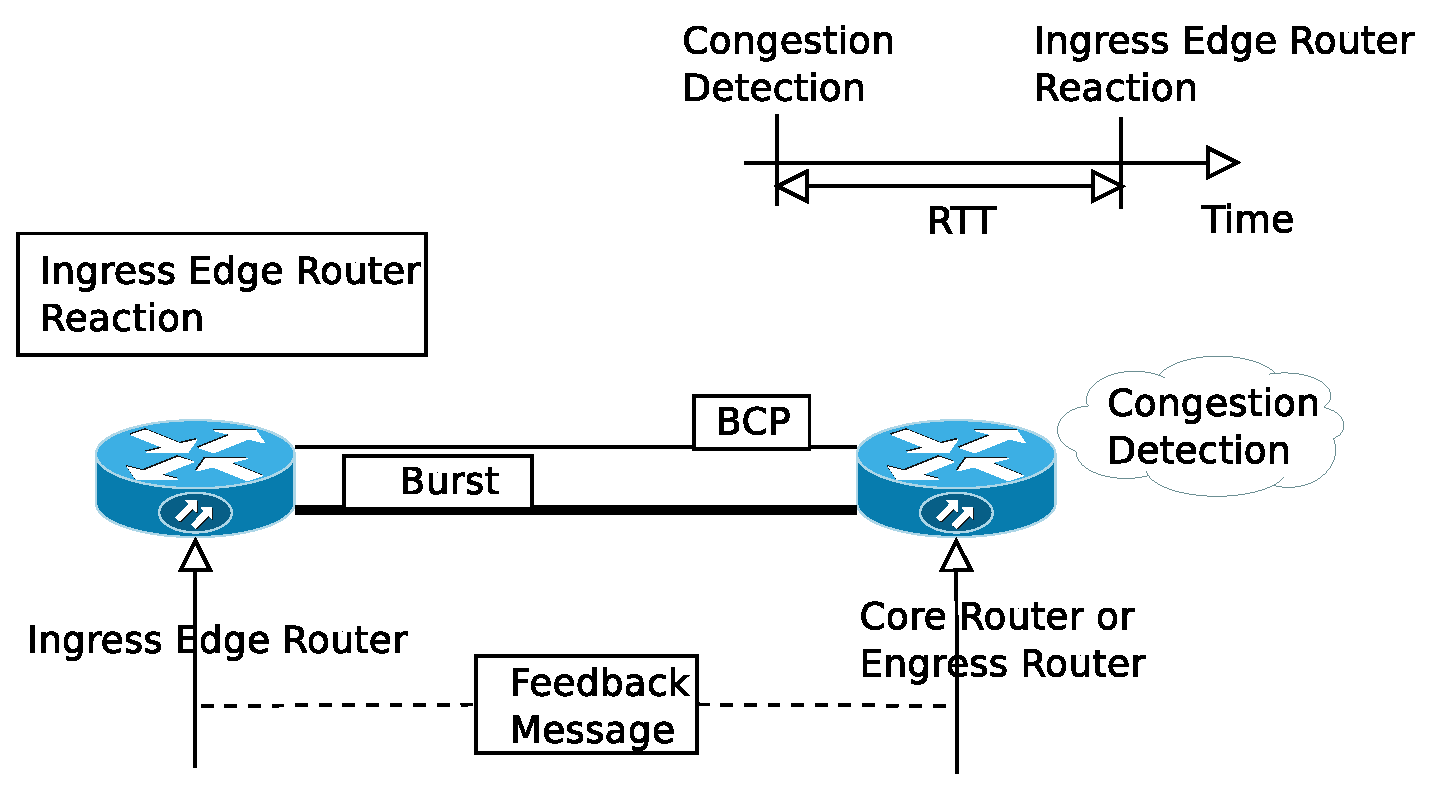
\includegraphics[height=6in]{pattern}}
        \else
        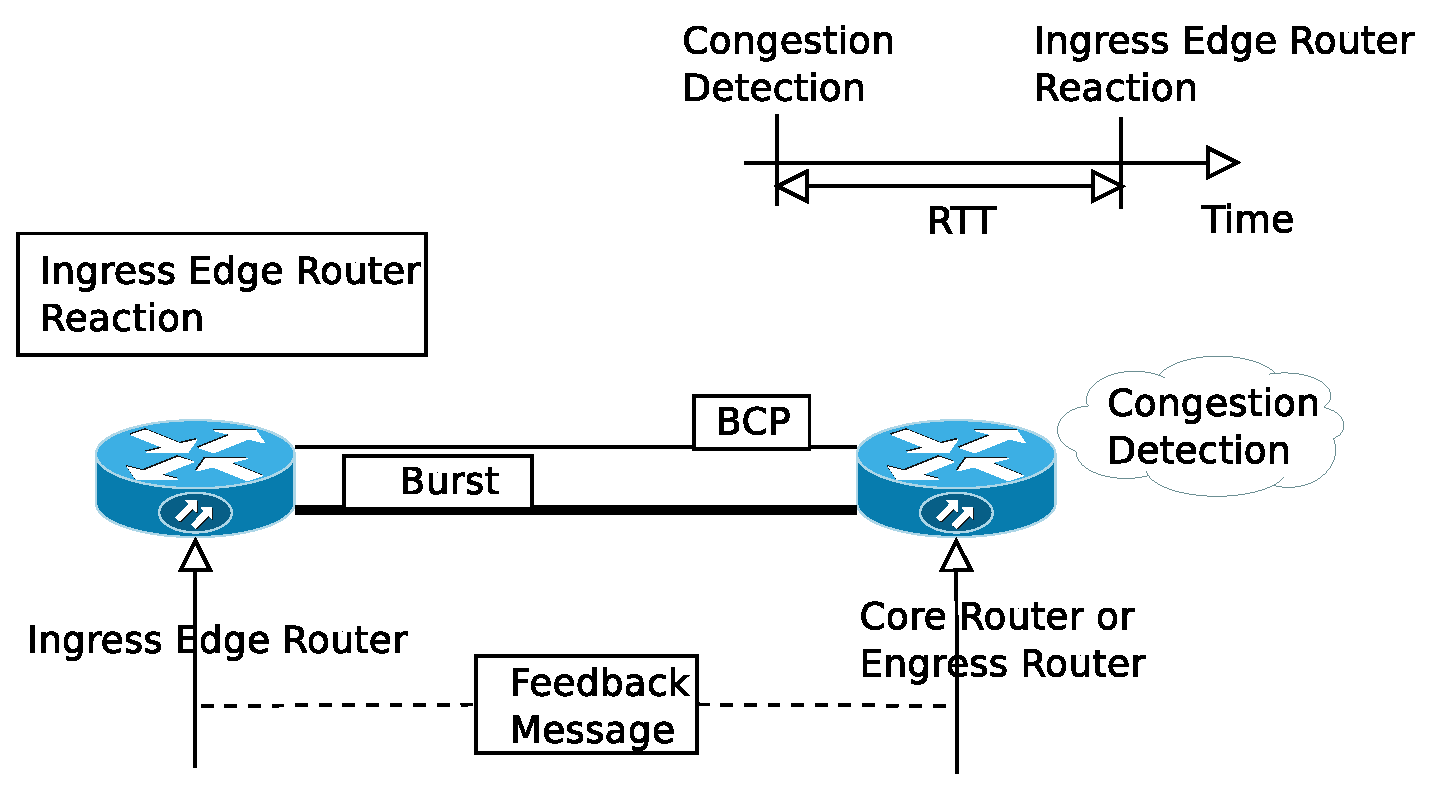
\includegraphics[bb = 92 86 545 742, height=6in]{pattern}
        \fi
        \caption{Pattern to control OBS congestion}
    \end{center}
\end{figure}

Figure \ref{fig:pattern} not only tell us the current popular pattern on research about OBS congestion control. It also tell us the steps to control congestion. This patter is practical and correct. So it will also be used in this study. Although the petter of vary congestion control mechanism are same. But there are a large amount difference among vary scheme in implementation detail. Such as different frequently to send feedback message to edge router, different way to
determine the congestion state threshold, different feedback message body. Certainly, they result in different performance. 

In their paper, they don't tell how to setup the threshold. They just give a final result. The value maybe have test a lot of times and they think that is proper for their model. It also is a constant value. But I think this value should adjust with the change of network topology. Besides, They don't tell how long is the RTT. The \verb|RTT| can use to measure the speed of ingress react. The \verb|Threshold| is a most important factor to affect the scheme to indicate congestion state or not.
But there is not a formula to got these two value through pure analysis. Current scheme just by trial and error to find a proper value for their simulation model.  

Moreover, Once their model is determined. All parameter is definite during simulation time. Include the most important \verb|Threshold| value. In my opinion, Congestion control is a dynamic optimization problem. This \verb|Threshold| should self-adjust accordingly. Burak Kantarci and Sema Oktug propose a congestion control scheme base on adaptive threshold \cite{adaptive}. The improvement is also very good. 

The previous researcher use throughput and loss ratio to measure their result. The higher throughput and the lower loss ratio. That will be propose as a better congestion control scheme. There also very important factor should be consider to determine whether a new scheme is better. That is whether as effective at high load as at low load. All previous researcher have pay much attention to this point. 

Previous mostly assume the burst arrive process follow the Poisson process and their lengths are negative exponentially distributed. But base on the some newest study. It has been shown that  whereas flow arrivals are Possion (or close to Possion), flow sizes are not exponential, but rather heavy-tailed, and thus they are closer to a Pareto distribution than an exponential one.  

\section{Issues May Encounter}

Note that in OBS networks, intelligent functions such as burst assembly, burst scheduling and generation of control packets are implemented at edge nodes while core nodes perform less complex functions such as processing control packets, resource reservation and switching bursts. However, many existing works have proposed to implementation some simple extra functions at the core node such as load calculation, burst segmentation and priority-based burst dropping for service differentiation.
It is hard to predict whether it is necessary to add extra function to core node in this study. If yes, is it complicate so that the core node is reject to add it.


To meet QoS requirement such as bounded delay or guaranteed delivery is part of new scheme objective. But it is incompatible to achieve guaranteed delivery rate and congestion control by reduce transmission rate at the same time. It is clear that even in ideal networks, where the switches use number of buffers and can perform wavelength conversion, congestion collapse still occurs when the load gets higher. On this moment, it seem impossible to resolve this contradiction.    

\section{Summary}

Overview the history of the development of OBS technology. The original goal is to compete with ATM network which have great potential in electronic domain. Compared with primitive Burst switching, ATM is more cost effective. But when WDM technology can provide huge bandwidth. It posed a challenge to current switch technology, that is how to use this bandwidth efficiently. The switch technology become the network bottleneck. OBS is a new technology that is currently
under study. It has not as yet been commercialized and standardized. But It has great potential to replace current switch technology. It has some advantages:

\begin{enumerate}
    \item More flexible and efficient compared with wavelength routed network
    \item More scalable and cost effective compared with opto-electronic approaches
    \item Smaller overhead and more practical compared with OPS
\end{enumerate}

It also have some prominent feature:

\begin{enumerate}

    \item Separation of transmission and control, Each user transmits data in bursts
    \item Basically, assumes the network is bufferless
    \item Network nodes(OXC) allocate resources for just this single burst

\end{enumerate}

By contrast, we can find that OBS has a lot of advantages for packet switch. However, unfortunately contention is inherent to the OBS technique. The contention problem is due to the lack of information at the nodes and the absence of global coordination between the edge routers and core routers. In one word, I want to proposed a new scheme to avoid and control congestion effectively in this study. And then drive OBS into standardized earlier.



%%% Local Variables: 
%%% mode: latex
%%% TeX-master: "../thesis"
%%% End: 

%\include{Chapter2/chapter2}
%\include{Chapter3/chapter3}
%\def\baselinestretch{1}
\chapter{Conclusions}
\ifpdf
    \graphicspath{{Conclusions/ConclusionsFigs/PNG/}{Conclusions/ConclusionsFigs/PDF/}{Conclusions/ConclusionsFigs/}}
\else
    \graphicspath{{Conclusions/ConclusionsFigs/EPS/}{Conclusions/ConclusionsFigs/}}
\fi

%\def\baselinestretch{1.66}

Up to now, we have know that DWDM take the bottleneck of networks from bandwidth to switching technology. OBS emerge as this requirement. OBS have many advantage with the advance of DWDM technology. It have great potential to be next generation switching technology in the core network. Since it have some special feature. Such as not require buffer, separation of transmission and control packet. 

As mention above chapter, contention is very possible occurs in ideal network without congestion control. OBS have no standardize yet. Many researcher work on this challenging topic. The main research method is simulation. Overview of all previous, they have build a theory framework to solve congestion collapse for OBS. That is three steps: detect, feedback, reaction. They are different in implementation detail. All mechanism are tightly coupled with the burst assembly mechanism at the
ingress edge router. This was decided by two reasons. The First is all intelligence resides in the edge router, which are at the same time the buffer and the processor. The second is the hurdle for congestion is lacking of communication between the nodes and the absence of global coordination between the edge routers and core routers. Hence, monitor on corn router and controller on edge router will be focus on the future work. 



%%% ----------------------------------------------------------------------

% ------------------------------------------------------------------------

%%% Local Variables: 
%%% mode: latex
%%% TeX-master: "../thesis"
%%% End: 


\backmatter % book mode only
%\appendix
%\include{Appendix1/appendix1}
%\include{Appendix2/appendix2}


%new
%\bibliographystyle{plainnat}
%endnew
\pagestyle{plain}
\bibliographystyle{Classes/CUEDbiblio}
%\bibliographystyle{Classes/jmb}
%\bibliographystyle{plainnat} %this works with package natbib
%\bibliographystyle{Classes/jmb} % bibliography style
\renewcommand{\bibname}{References} % changes default name Bibliography to References
\bibliography{References/references} % References file

\end{document}
